%-------------------------------------------
\begin{frame}{Really need of a files history?}
%-------------------------------------------
\begin{columns}
  \column{0.5\textwidth}
  \begin{center}
        \href{http://phdcomics.com/comics/archive.php?comicid=1531}{
\includegraphics[height=8cm]{05_history/Images/FAIR_git_comic_phd101212s.png}}
  \end{center}
  \column{0.5\textwidth}
  \begin{center}
     \textit{“Most researchers are primarily collaborating with themselves,” [Tracy] Teal explains. “So, we teach it from the perspective of being helpful to a ‘future you’." }
   \end{center}
\end{columns}
\end{frame}
%-------------------------------------------
\begin{frame}{Files history = good practice for reproducible research}
%-------------------------------------------
\begin{center}
    \textit{"Rule 4: Version Control All Custom Scripts"}\\
    \href{https://journals.plos.org/ploscompbiol/article?id=10.1371/journal.pcbi.1003285}{
\includegraphics[height=5cm]{05_history/Images/FAIR_10simplesRules.png}}
\end{center}
\end{frame}
%-------------------------------------------
\begin{frame}{Version control}
%-------------------------------------------
\begin{columns}
  \column{0.6\textwidth}
   \begin{block}{Definition}
version control, revision control, source control, or source code management: class of systems responsible for managing changes to files.
   \end{block}
   \begin{block}{Feature}
Each revision is associated with a timestamp and the person making the change. \\
Revisions can be compared, restored, and merged.
   \end{block}
   \begin{block}{Software}
   SVN, Git, Mercurial, GNU arch, etc
   \end{block}
   \href{https://en.wikipedia.org/wiki/Version_control}{\textcolor{blue}{\underline{wikipedia source}}}
 \column{0.3\textwidth}
   \begin{block}{Revisions graph}
   \begin{center}
      \href{https://en.wikipedia.org/wiki/File:Revision_controlled_project_visualization-2010-24-02.svg}{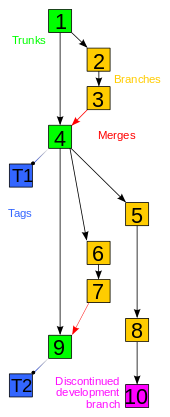
\includegraphics[height=7cm]{05_history/Images/FAIR_git_revision_graph_wikipedia.png}}
   \end{center}
   \end{block}
\end{columns}
\end{frame}
%-------------------------------------------
\begin{frame}{Git and GitHub}
%-------------------------------------------
\begin{columns}
 \column{0.48\textwidth}
   \begin{block}{Git}
   \begin{center}
       
\includegraphics[height=2cm]{shared/logo-git.png}
   \end{center}
   \begin{itemize}
       \item will track and version your files
       \item enables you to collaborate with ... yourself
       \item open source license GPL (GNU General Public License)
       \item created in 2005 by Linus Torvalds for the development of the Linux kernel
   \end{itemize}
\end{block}
 \column{0.48\textwidth}
 \begin{block}{GitHub}
 \begin{center}
      
\includegraphics[height=2cm]{shared/logo-github.png}
 \end{center}
  \begin{itemize}
      \item stores your \raisebox{-0.5ex}{
\includegraphics[height=0.4cm]{shared/logo-git.png}} repositories online
      \item enables you to collaborate with others (and yourself)
      \item first commit in 2007 by Chris Wanstrath, founded in feb. 2008, Microsoft Corporation still 2018
  \end{itemize}
\end{block}
\end{columns}
\end{frame}